\documentclass[titlepage]{article}

\usepackage[utf8]{inputenc}
\usepackage{graphicx}
\usepackage{listings}
\usepackage[bookmarks=true]{hyperref}
\usepackage[all]{hypcap}        % needed to help hyperlinks direct correctly;

\title{SongBook\\ \large Application programming – Java and XML technologies}
\author{Michał Kowalski\\Maciej Borkowski}
\date{}

\begin{document}
\maketitle

\section{Introduction}
SongBook is, without a surprise, a song book. It allows users to see lyrics and
chords for songs (for example for guitar learning purposes), grouped by
artists/authors, stored in application's directory in XML format. Adding/deleting/modifying of songs/artists can be done by
adding/deleting/modyfing proper XML files. Application is written in Java, using
JAXB and Swing.

\section{Data model}
All application's data is stored in 3 types of XML files:
\begin{itemize}
  \item index files,
  \item artist files,
  \item song files.
\end{itemize}
All types of files are parsed using JAXB into instances of classes. All of them,
except index ones, are loaded on-demand (lazy loading), which reduces application's start time and required memory, when database grows, and allows
for changing data at runtime. Other exception with index files is that it is
possible to have many index files, and result is the same as having all data in
only one. Other types must have whole content in one file. 

\subsection{Index file}
Index file, as shown on fig. \ref{lst:index}, contains a list of artist entries.
Each entry contains a name of artist and its ID. To find a data for artists,
file name must be equal to artist's ID. Index file and artist entry have their
appropiate Java classes for binding purposes.

\begin{figure}
\lstinputlisting[breaklines=true]{../test_db/index1.xml}
\caption{Example file containing list of authors}
\label{lst:index}
\end{figure}

\subsection{Author file}
Author/artist file, as shown on fig. \ref{lst:artist}, contains a list of song
entries and a description of author. Song entry contains song name and ID, and
latter of those two is used for finding file with data for each song. Author
file and song entry have their appropiate Java classes for binding purposes.

\begin{figure}
\lstinputlisting[breaklines=true]{../test_db/artists/jenny_donelly.xml}
\caption{Example file for author containing list of his songs}
\label{lst:artist}
\end{figure}

\subsection{Song file}
Song file, shown on fig. \ref{lst:song}, is lowest file in data hierarchy. This
file contains data for song - its lyrics and chords, represented in Java as
simple list of strings, so only file must have own class for binding.

\begin{figure}
\lstinputlisting[breaklines=true]{../test_db/songs/song_a.xml}
\caption{Example file for song}
\label{lst:song}
\end{figure}

\section{GUI}
Main goal of designing GUI was to keep it simple. Actions available to user are:
\begin{itemize}
  \item choosing artist from list,
  \item choosing song for chosen artist
  \item choosing side-by-side or alternate displaying of lyrics and chords of
  songs
\end{itemize}
When user chooses artist using combo-box, song's combo-box is repopulated with
titles of songs belonging to that artist. In next step user chooses
song, and its lyrics and chords appear in text area. User can choose between two
ways of displaying them:
\begin{enumerate}
  \item Side-by-side - when user prefers to see chords next to lyrics.
  \item Alternately - when user prefers to see chords for lyrics above each
  line, or song doesn't have one of them, so showing two columns will be a waste
  of space.
\end{enumerate}
In side-by-side way of showing it's important to always have proper lines next
to each other, so when all lines don't fit into current window size, they are
scrolled using one scrollbar.

\begin{figure}
\centering
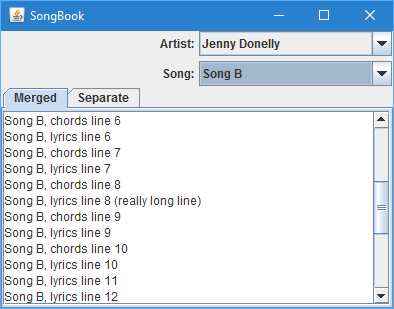
\includegraphics{img1}
\caption{Application displaying lyrics and chords alternately}
\label{img:merged}
\end{figure}

\begin{figure}
\centering
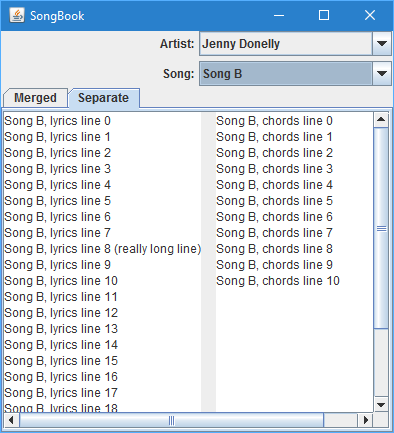
\includegraphics{img2}
\caption{Application displaying lyrics and chords side-by-side}
\label{img:separate}
\end{figure}

\end{document}